% -*- coding: utf-8 -*-
%%
%%  本模板可以使用以下两种方式编译:
%%     1. PDFLaTeX
%%     2. XeLaTeX [推荐]
%%  注意:
%%    1. 在改变编译方式前应先删除 *.toc 和 *.aux 文件,
%%       因为不同编译方式产生的辅助文件格式可能并不相同。

%\documentclass{cumcmart}
\documentclass[nocover]{cumcmart}%%
%切换到无封面的版本,有些赛区不允许前面的承诺页用pdf格式,可以用此选项去掉。

%\usepackage[refsection=section]{biblatex}
\usepackage{listings}
\usepackage{cite}
\begin{document}


\title{关于同心鼓游戏获胜策略的研究}

\xuanti{A}
%\school命令用于在承诺书上显示学校名称。按要求,此处应填写全称
\school{XXXX大学}
%以下命令分别显示队员及指导教师姓名
\numbers{2010888}%参赛报名号
\authorone{队员1}
\authortwo{队员2}
\authorthree{队员3}
\advisor{数模指导组}

\newcommand{\lhp}[1]{\textcolor{cyan}{lhp: #1}}
\newcommand{\znq}[1]{\textcolor{blue}{znq: #1}}

%\theyear{2010}

\theday{16}%填写当月的具体日期

\maketitle
\begin{cnabstract}%此处没有采用sbstract命名,是为了将来如果要加入英文摘要时扩展的方便

摘要在这里


\cnkeywords{关键词;关键词}
\end{cnabstract}

\newpage
%\tableofcontents\newpage%增加目录,要不要都可以。不想要的话,就在本行前加“%”(英文的百分号)


\section{问题重述}
\subsection{问题背景}
“同心协力”(又称“同心鼓”)项目考察团队协作能力。该项目要求团队成员使用一牛皮双面鼓,鼓身一圈固定多根长度相同的绳子,绳子的固定点沿圆周均匀分布。每条绳子的另一头由一位团队成员牵拉,控制整条绳,并通过绳子共同控制鼓。

项目开始时,球从鼓面中心上方竖直落下,队员共同控制绳子,让鼓将球颠起,使其有节奏地在鼓面上跳动。颠球过程中,队员只能抓握绳子的末端,不能接触鼓或绳子的其他位置。

项目所用排球的质量为 270 g。鼓面直径为 40 cm,鼓身高度为 22 cm,鼓的
质量为 3.6 kg。队员人数不少于 8 人,队员之间的最小距离不得小于 60 cm。项目开始时,球从鼓面中心上方 40 cm处竖直落下,球被颠起的高度应离开鼓面 40 cm 以上,如果低于 40 cm,则项目停止。试探索策略,使得项目结束时,总共颠球次数尽可能的多。

\subsection{提出问题}
问题1:在理想状态下,每个人都可以精确控制用力方向、时机和力度,试讨论
这种情形下团队的最佳协作策略,并给出该策略下的颠球高度。

问题2:在现实情形中,队员发力时机和力度不可能做到精确控制,存在一定误
差,于是鼓面可能出现倾斜。试建立模型描述队员的发力时机和力度与某一特定
时刻的鼓面倾斜角度的关系。设队员人数为 8,绳长为 1.7m,鼓面初始时刻是水
平静止的,初始位置较绳子水平时下降 11 cm,表 1 中给出了队员们的不同发力
时机和力度,求 0.1 s 时鼓面的倾斜角度。

问题3:在现实情形中,根据问题 2 的模型,对问题1中的模型进行合适的调整。

问题4:当鼓面发生倾斜时,球跳动方向不再竖直,于是需要队员调整拉绳策略。
假设人数为 10,绳长为 2m,球的反弹高度为 60cm,相对于竖直方向产生 1 度
的倾斜角度,且倾斜方向在水平面的投影指向某两位队员之间,与这两位队员的
夹角之比为 1:2。为了将球调整为竖直状态弹跳,请给出在可精确控制条件下所
有队员的发力时机及力度,并分析在现实情形中这种调整策略的实施效果。

\section{问题分析}
在同心鼓游戏中,为了使颠球的次数尽可能的多,多位团队成员需要齐心协力,尽可能使鼓表面保持水平。因此,团队成员应当尽量将每次颠球的发力时机控制在同一时刻。并且,在球距离鼓面高度需大于40cm的条件下,团队成员应当尽量将球的颠起高度控制在40cm,不需要过高,以节省力气,保证更多的颠球次数。

对于问题1,我们考虑每个人都可以精准控制用力方向、时机和力度的理想状况。为了使颠球次数尽可能多,我们要求团队成员每次将球颠起的高度恰好为40cm,即合法的最小高度。这是一个最节省能量的方案,我们也将此认定为最优方案。

对于问题2,考虑到实际情况下,某些人发力的时间和力度可能会有一定误差,我们计算误差情况时,对鼓的表面所造成的倾斜影响。在此问题中,首先计算鼓的转动惯量,然后使用角动量定理计算出鼓的角加速度。在此基础上,我们列出动力学方程,计算鼓面的转动角度。



\section{模型假设}

\begin{enumerate}
    \item 不考虑球的形状与体积,将球视为质点。
    \item 不考虑绳的弹性与质量,将绳视为轻绳。
    \item 不考虑鼓上表面的曲率,将鼓上表面视为二维平面。
    \item 不考虑球和鼓运动过程中的空气阻力。
    \item 将鼓视为薄壁圆桶。
    \item 假设每个人牵拉绳时手的位置在同一平面上。
    \item 假设每条绳子的固定点到牵拉者手的距离相同。
    \item 假设任意相邻两条绳子所成的夹角相同。
\end{enumerate}

\section{符号}
我们在\ref{table:symbol}此列出本文中会用到的所有符号,并声明其含义。
\begin{table} [!h]
\begin{center}
\vspace{-0.1in}
\caption{本文中用到的符号}
\label{table:symbol}
\begin{tabular}{|c|l|}
\hline
\textbf{符号}&\textbf{含义}\\
\hline
$e$&球和鼓面碰撞后的恢复系数\\
\hline
$I$&鼓面的转动惯量\\
\hline
$v_0$&球与鼓面碰撞后的初速度\\
\hline
$M$&鼓的质量\\
\hline
$m$&球的质量\\
\hline
$\beta$&受到外力时鼓面的角加速度\\
\hline
$\delta$&外力对鼓面造成的旋转角度\\
\hline
$\omega$&鼓面转动的角速度\\
\hline
$T$ &整个过程的周期\\
\hline
$\theta_i$ &第$i$条绳与y轴的夹角\\
\hline
bias &$\theta_i - \frac{\pi*i}{4}$\\
\hline
\end{tabular}
\vspace{-0.2in}
\end{center}
\end{table}


\section{模型建立与求解}
\subsection{问题1:最理想状态}
\subsubsection{建立模型}
在理想状态下,我们假设每个人的发力时间和力度都可以被精准控制。因此,我们首先要求所有人的发力时间一直,力度大小相同。在此基础上,
考虑最优解,我们认为题意对于球上升高度的要求是指球与鼓之间的相对高度差不低于0.4m,因此选取使得球弹起最小的高度,即球与鼓之间的相对距离的最大值为0.4m,显然这是一个最节省能量的方案。除此之外,由于球上升的距离最小,这个运动的周期也是最小的,这也可以在单位时间内进行弹起最多的次数。

我们在这里建立如下的模型:

所有人围成一圈,使得每个人抓住绳子的手的位置均匀分布在一个正多边形的各个顶点。绳子另一端均匀分布在鼓的四周,将之抽象为图\ref{5.1.1 模型抽象示意图}所示。
\begin{figure}[h!]
    \centering
    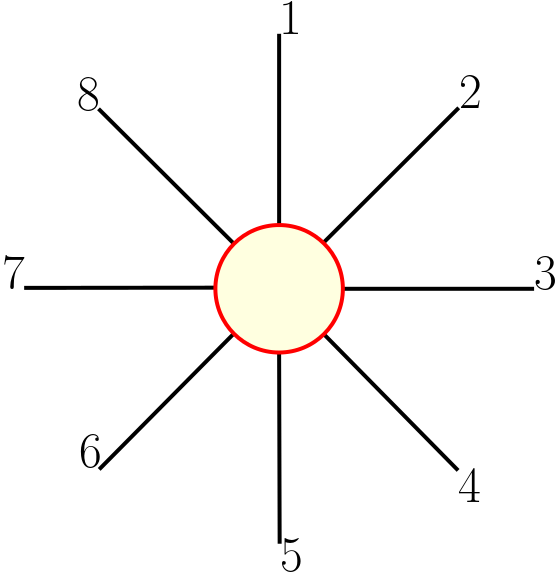
\includegraphics[width=0.4\linewidth]{figures/f1.png}
    \caption{5.1.1 模型抽象示意图 (8人情况)}
    \label{5.1.1 模型抽象示意图}
\end{figure}

我们首先分析球的一系列运动。球每次与鼓碰撞之后,首先进行竖直上抛运动,当速度减为0时,再进行自由落体运动。当球落下至初始位置时,会与鼓再次相碰,重复刚才的一系列运动。
球的运动是周期运动。

我们接下来分析鼓的一系列运动。鼓每次与球碰撞之后,首先进行竖直上抛运动,当速度减为0时,再进行一段自由落体运动。该过程绳子保持松弛。当绳子绷紧时,自由落体运动结束,
随后由于团队成员所施加外力的影响,鼓在某一位置$y_{d1f}$开始进行加速度恒定、方向竖直向下的匀减速直线运动,直至速度减为0。接下来,由于团队成员所施加外力的影响,鼓以相同的加速度进行向上的匀加速直线运动,到达碰撞的位置,与球进行碰撞。
鼓的运动也是周期运动。

在此模型中,我们假设所有团队成员在相同的时刻,位于相同的高度拉绳子,并在鼓与绳子碰撞的瞬间松开绳子使其自由落体。此外,所有团队成员均能够准确的控制拉绳子的力与时间,并且同一时刻每个团队成员施加的力大小相等,与竖直方向所成的夹角相等。在求得鼓与球的运动学规律之后,我们可以基于此假设求得每个团队成员在整个过程中任意位置的力的大小与方向。
\subsubsection{模型求解}
现在我们对该模型进行求解。

\begin{enumerate}[(a)]
\item
球与鼓运动周期的时间记位$T$,则
$$T = \frac{2v_0}{g}$$
    \item
    鼓竖直上抛的过程经过t1结束,则
    $$y_{d1f} = v_{1i}t1 - \frac{1}{2}g t_1^2$$
    $$v_{1f} = v_{2i} = v_{1i}-gt1$$
    \item
    鼓进入匀加速直线运动状态,经过t2回到初始状态,
    $$0 = y_{d1f} + v_{2i}t2 + \frac{1}{2}a t_2^2$$
    鼓与球之间的最大距离为$\Delta H = 0.4$m,
    $$\Delta H = (v_0 - v_{1i})t1 + \frac{(v_0 -v_{1i})^2}{2(g+a)}$$
    $$v_{2f} = v_{2i} + a_2 t_2$$
    $$T = t1 + t2$$
    \item
    考虑碰撞的过程,设恢复系数为e,则考虑动量守恒与恢复系数的定义可以得到
    $$m v_0 + M v_{1i} = M v_{2f} - m v_{0}$$
    $$v_0 - v_{1i} = e(v_0 + v_{2f})$$
    \item
    不妨设绳长为L,球与鼓发生碰撞的位置距离团队成员手所在的平面$h_0$,不妨以竖直向上为正方向,当鼓位于$y_d$时,由于拉力必然沿绳方向,故拉力与水平面的夹角为(以向上的角为正),
    $$\theta = \arcsin{\frac{y_d - h_0}{L}}$$
    拉力满足动力学方程,
    $$n T \frac{-y_d}{L}-Mg = Ma$$
    解得,
    $$T = \frac{-ML(a+g)}{n (y_d - h_0)}$$
    \znq{麻烦你在Problem1.m中添加上式的代码,求得几个位置的拉力T的大小,可以假定$n, h_0, L$ 等参量,$y_1$ -0.01~-0.06,$e$ 0.4~0.9}
    此处当鼓与球相碰之后,T将小于0,但是此时鼓处于竖直上抛的状态,因而此矛盾不存在。
\end{enumerate}

我们根据一定的化简之后,使用MATLAB求其数值解,求解代码如附件Problem1.m所示。
我们不妨对于$e = ?, n = 8$为例进行求解,
可得

\znq{我在这里想要一个表格,代表不同e的情况下,求得的各个参量的结果}

\znq{注意这一问在问球能够弹多高,不要在表格中落了这一项}

\subsection{问题2:非理想状态,计算短时间内鼓面倾斜角度}
\subsubsection{建立模型}
由于鼓受到团队成员拉绳的作用时间与力的大小存在差别,其在质心运动的同时,也会收到一个相对于质心的净力矩,因此鼓面会产生一定大小的角速度,与初始状态所在平面产生一定夹角。在产生夹角的同时,每根绳的受力方向也可能发生变化。我们考虑外力对鼓的质心所产生的力矩,计算出来鼓旋转的角加速度,进而使用时间微元法,认为在每一微元时间内,角度,角速度,角加速度均为定值。

该过程分析如下:

\begin{enumerate}[(a)]
    \item 
计算转动惯量$I$:

我们将鼓视为匀质薄壁圆筒,同时忽略上下表面(鼓皮)的质量。同时根据题目图片所示,我们假定绳子连接在鼓侧壁母线的中点处,我们假设鼓的旋转就是沿着母线中点所在水平轴的旋转,这一轴同时通过质心,由此建立坐标系,求鼓相对于此轴的转动惯量$I$,具体代码如I.m所示。

\znq{来一个超链接至附录的I.m的位置}

$$I = \iint dm(y^2 + z^2) = \iint  rd\theta dz (z^2 + r^2 \sin{\theta}^2) = 0.0865 kg\cdot m^2$$
\item 估算只有一个力,经过0.1s可以对于鼓产生的影响,
\begin{enumerate}
    \item 假设旋转角度较小,可以忽略力水平分量对于旋转轴的力矩,只考虑力竖直分量产生的影响,此时,
    $$\vec{M} = \vec{r}\times \vec{F}$$
    $$|\vec{M}| = rF\alpha = 1.035 N\cdot m$$
    \item 根据角动量定理,此时的角加速度为
    $$\beta = \frac{M}{I} = 11.97 s^{-2}$$
    \item 假设其匀角加速度运动,在0.1s内可以转过的角度为
    $$\delta = \frac{1}{2}\beta \Delta t^2 = 0.06 rad$$
    \item 由此可见,这个角度与其所受拉力与水平面的夹角相比,仍然是一个很小的量,这意味着我们之前忽略力水平分量的假设是合理的。
\end{enumerate}
\end{enumerate}

由此我们可以看出,在加速的第一阶段,旋转角达到最大时,也只有0.06 rad,该角度依然很小。由于鼓的半径与绳子的长度相比很小,我们便可以忽略在这个过程中,力的方向的变化。我们计算的过程允许了非小角的存在,因此即使算出较大的旋转角,也是合理的结果。

因此,我们建立如下的模型:

我们将产生误差的情况分为两种:对称的情况与非对称的情况。对称的情况定义如下:拉绳时间不同与拉绳力度不同在同一方向发生。在这种情况下,两种误差所带来的影响是同方向的,我们可以认为鼓围绕某一轴做定轴转动;非对称的情况定义如下:拉绳时间不同与拉绳力度不同在不同方向发生。在这种情况下,两种误差所带来的影响是不同方向的,我们应该研究刚体的定点转动。

\subsubsection{模型求解}
我们首先求解对称的情况,这种情况下鼓进行定轴转动。
不妨根据定轴转动的轴对于不同的受力点进行编号。此处我们将定轴转动的轴规定为拉力对称轴通过圆心的垂线。在此基础上,我们建立三维坐标系:$y$轴为旋转轴,正方向朝向纸面外;$z$轴垂直于鼓面初始状态所在平面,正方向为竖直向上;$x$轴由$y$轴、$z$轴共同确定,三条轴的分布满足右手定则。

利用在问题1中已经求得的转动惯量,我们列出如下的动力学方程
$$|\sum_{i = 1}^{n} \vec{M_i}| = I\frac{d\omega}{dt}$$

不妨设鼓面转过角度为$\delta$。在建立模型时,我们已经证明了角度转动很小,但是为了得到更加准确的结果,我们仍然考虑不同位置的不同$\delta$的情况。
$$\omega = \frac{d\delta}{dt}$$

此处的代码我们用到了一个变量bias。这里的bias定义为
$$bias = \theta_i - \frac{\pi*i}{4}$$
即每条绳子与其所对应的原始位置的角度之差。

现在我们计算每一条绳子受力点的坐标与三个方向上的受力情况。

$$\vec{r_i} = (r\sin{\theta_i}\cos{\delta}, r\cos{\theta_i}\cos{\delta}, r\sin{\delta})$$
$$\vec{F_i} = (F\sin{\theta_i}\cos{\alpha}, F\cos{\theta_i}\cos{\alpha}, F\sin{\alpha})$$
$$\vec{M_i} = \vec{r_i} \times \vec{F_i}$$
这里我们使用微元法,将时间分割成小时间段的方法进行数值模拟,即
$$\omega(t+\Delta t) = \omega(t) + \frac{|\sum_{i = 1}^{n} \vec{M_i}|}{I} \Delta t$$
$$\delta(t+\Delta t) = \delta(t) + \omega \Delta t$$
只需要求出每个位置的总力矩,就可以对其进行数值模拟,代码如附件Problem2.m所示

\znq{这里跑一下Problem2.m,输入的F, activate, bias等数据位于Prob2data.txt文件中}
计算结果如\ref{table:result}所示。其中,序号顺序与题目一致。我们规定,如图所示,以旋转轴朝向纸面外的方向为$y$轴正方向,以满足右手定则朝向$y$轴正方向的旋转方向为旋转的正方向。计算结果中,正值为旋转正方向的同方向,负值为旋转正方向的反方向。
\begin{table} [!h]
\begin{center}
\vspace{-0.1in}
\caption{计算结果}
\label{table:result}
\begin{tabular}{|c|l|}
\hline
\textbf{序号}&\textbf{鼓面倾角 (rad)}\\
\hline
1&-0.0797\\
\hline
2& -0.1694\\
\hline
3& -0.0587\\
\hline
4&-0.5492\\
\hline
5&-1.2531\\
\hline
6&-0.3953\\
\hline
7&-1.0126\\
\hline
9&0.2946\\
\hline
\end{tabular}
\vspace{-0.2in}
\end{center}
\end{table}     

\subsubsection{模型分析}
我们发现大多数的情况下旋转角是一个较小的角度,而在5和7。。。
\znq{补充一下}

\subsection{问题3:现实情形,考虑较长时间内鼓面的倾斜}
\subsubsection{建立模型}

鼓进入匀减速直线运动的过程时的速度为$v_{2i} = -0.60 ms^{-1}$,位置为$y_{d1f} = -0.01m$,加速度为$a = 3.0ms^{-2}$,因此再经过$\delta t = -\frac{v_{2i}}{a} = 0.2s$后,鼓到达最低位置,此位置为

$$y_{dlow} = y_{d1f} + v_{2i}\delta t + \frac{1}{2}at^2 = -0.06m$$
这意味着整个过程中鼓最多相对碰撞位置下降6cm,这与问题2中的11cm同量级,我们可以借助问题2的方法,认为在此问题中鼓处于14cm处,便可以得到一个同量级的估算结果。

我们发现,如果不加任何修正,对于问题2中的情形,如果沿用问题1中建立的模型,由于0.1s后残余的可观的角速度,经过长达0.5s量级的旋转,会在下一次碰撞前达到巨大的旋转角度,继而将球碰偏。为了解决这个问题,我们努力减少碰撞前转过的角度,并尽量减少碰撞时其旋转的角速度,尽最大可能减少其对于碰撞的影响,同时消减其对于下一周期所产生的消极影响。

问题3与问题2不同的是,当考虑系统长时间的过程时,可观的角速度可能使其旋转角度不可忽略,这意味着在大角度情况下,无法忽略拉力的水平分量产生的力矩。在水平分量产生的力矩可以被忽略时,为了消除已经发生的旋转,理所当然的应该减少对应方向的力,以产生总的恢复力矩。但是对于非小角的情况,考虑水平分量产生的力矩,则应该加大对应方向的力,以增大其水平分量,以得到更大的恢复力矩。此外,经过问题2中的实验,产生角度差别的主要原因不是力量的少许不同,更大程度上受到开始施力的时间不同的影响。

\znq{reference:0.2s那里加}

我们假设人可以分辨鼓朝向其方向旋转或朝向其反向旋转,可以分辨鼓旋转的速度为快或慢,可以选择加大力度或减少力度,分别对应着加大或减少50\%的力。由于人的视觉反应时间为0.2s左右,提早发力的人可以在0.2s后发现。因为单个或者是两个人增大力量对于总体的合力的影响并不大,所以质心的运动仍然可以使用问题1中的模型。根据问题1的模型,可以发现为了维持不变的加速度,不同位置的拉力在同一个数量级中变化,因此可以近似将它们套用问题2中的模型。

具体而言,将拉绳的过程分成三个部分,策略如下,

\begin{enumerate}
    \item -0.1s到0s
    
    提早拉绳的人进行拉绳
    \item 0s到0.1s
    
    所有人正常拉绳
    \item 0.1s到0.4s
    
    0.1s时,提早拉绳的人发现了自己的失误,由于其提早拉绳,一般而言鼓将背对其运动,对于鼓的状态进行判断,
    \begin{enumerate}
        \item 如果鼓背向自己旋转,且旋转速度快:加大力度
        \item 如果鼓背向自己旋转,且旋转速度很慢:减少力度
        \item 如果鼓朝向自己旋转,则保持原状态(这意味着相对的方向的人也出现了失误,避免了双方修正所带来的冗余)
    \end{enumerate}
\end{enumerate}

\subsubsection{模型求解}
仍然使用问题2中所用的时间微分法与问题2中的模型,由于问题2中考虑了夹角非小角的情况,我们的计算在较大旋转角的情况下,也是合法的。我们在此选取了问题2中的第5组数据为例,这里使得其增大力量50\%,进行微元法数值模拟,考虑不同时间的旋转角、角速度、角加速度等运动学参量,并由此得出较为真实的运动特征,具体计算代码如Problem3.m所示。

\znq{麻烦用问题2的数据再代入问题3的模型求一遍最后的偏转角}
\subsubsection{模型分析}
我们发现对于不同的情况,采用我们的策略均能够得到较好的效果,在这个运动过程中,鼓面会在一个较小的范围内运动,最终能够在要求时间内较为稳定地达到几乎水平的状态,这样只需要较小的位移便可以实现连续垫球不掉落。于此同时,这种方案可以保证最终状态的角速度较小,继而当球不精准落在鼓心时,可以减少对于球的运动所造成的影响。我们的模型还考虑了心理学与神经科学的研究结果,可操作性较强。

在实验中我们惊喜地发现,我们策略产生的结果对于初始状态与结束时间不敏感,这是一个十分优良的性质。有了这条性质,便可以在一定程度上弥补人的反应时间的影响,并且可以适应更多不同的情况。

\subsection{问题4:特殊情况:给定条件下的鼓面调整}


\section{模型的检验}
\section{进一步讨论}
\section{模型的优缺点}









\bibliographystyle{plain}
\bibliography{reference}
\newpage
\appendix
\section*{附录}
\begin{appendix}
\section{1}
x
\section{问题2代码}
\lstset{breaklines}
\begin{lstlisting}[language=Matlab,numbers=left, numberstyle=\tiny,keywordstyle=\color{blue!70},commentstyle=\color{red!50!green!50!blue!50},frame=shadowbox, rulesepcolor=\color{red!20!green!20!blue!20}] 
% 以对称轴为y轴,则各个力位于(4i/pi + bias)的位置
F = [90,80,80,90,80,80,80,80];
activate = [0,0,0,0,1,0,0,1];
bias = -pi/8;
theta = [];
I = 0.0865;
for i = 1:8
    theta(1,i) = pi*i/4 +bias;
end
alpha = 0.11/1.7;
delta = 0;
omega = 0;
% first period
for i = 1:10000
    M = [0,0,0];
    for j = 1:8
        r = [0.2*sin(theta(1,j))*cos(delta), 0.2*cos(theta(1,j))*cos(delta),0.2*sin(delta)];
        Fj = [F(1,j)*sin(theta(1,j))*cos(alpha), F(1,j)*cos(theta(1,j))*cos(alpha), F(1,j)*sin(alpha)];
        if activate(1,j)==1
            M = M + cross(r,Fj);   
        end
    end
    delta = delta + omega* 0.1/10000;
    omega = omega + M(1,2)/I * 0.1/10000;
end
%second period
for i = 1:(30000)
    M = [0,0,0];
    for j = 1:8
        r = [0.2*sin(theta(1,j))*cos(delta), 0.2*cos(theta(1,j))*cos(delta),0.2*sin(delta)];
        Fj = [F(1,j)*sin(theta(1,j))*cos(alpha), F(1,j)*cos(theta(1,j))*cos(alpha), F(1,j)*sin(alpha)];
        % r
        % Fj
        M = M + cross(r,Fj); 
    end
    delta = delta + omega* 0.1/10000;
    omega = omega + M(1,2)/I * 0.1/10000;
end
omega
delta
\end{lstlisting}
\end{appendix}

\end{document}
